\clearpage
\section{Noise Reduction in the Spatial Domain}


\subsection{Section0}
\begin{figure}[ht]
\centering
	\subfigure[Original image]{
	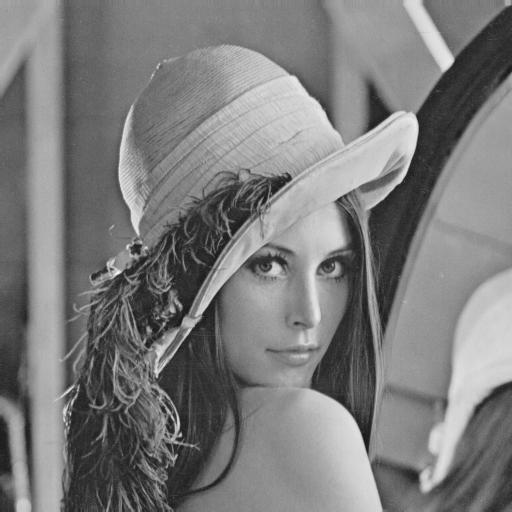
\includegraphics[width=0.45\linewidth]{question3/0_lenaBase}
	}
	\subfigure[Histogram]{
	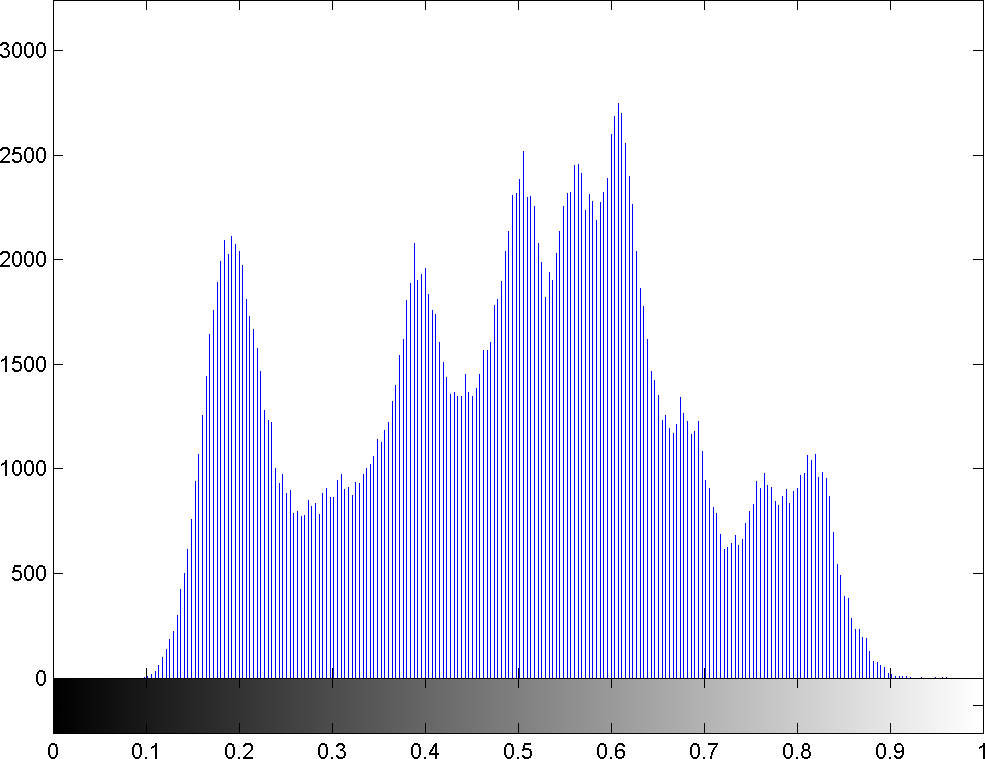
\includegraphics[width=0.45\linewidth]{question3/0_lenaBase_hist}
	}
	\subfigure[Image with Gaussian noise $\mu$=0, $\sigma^2$=0.002; PSNR +26.99dB]{
	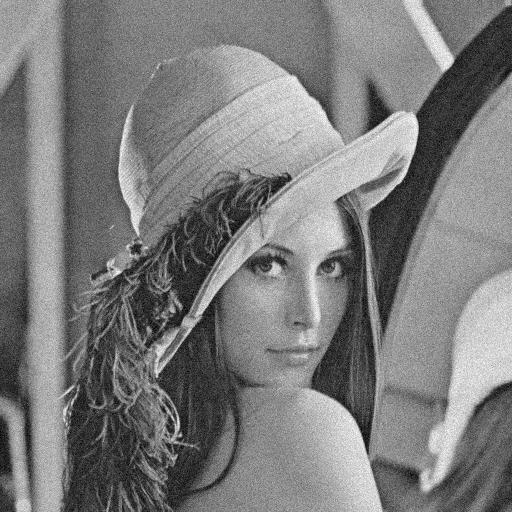
\includegraphics[width=0.45\linewidth]{question3/0_lenaNoisyGauss}
	}
	\subfigure[Histogram]{
	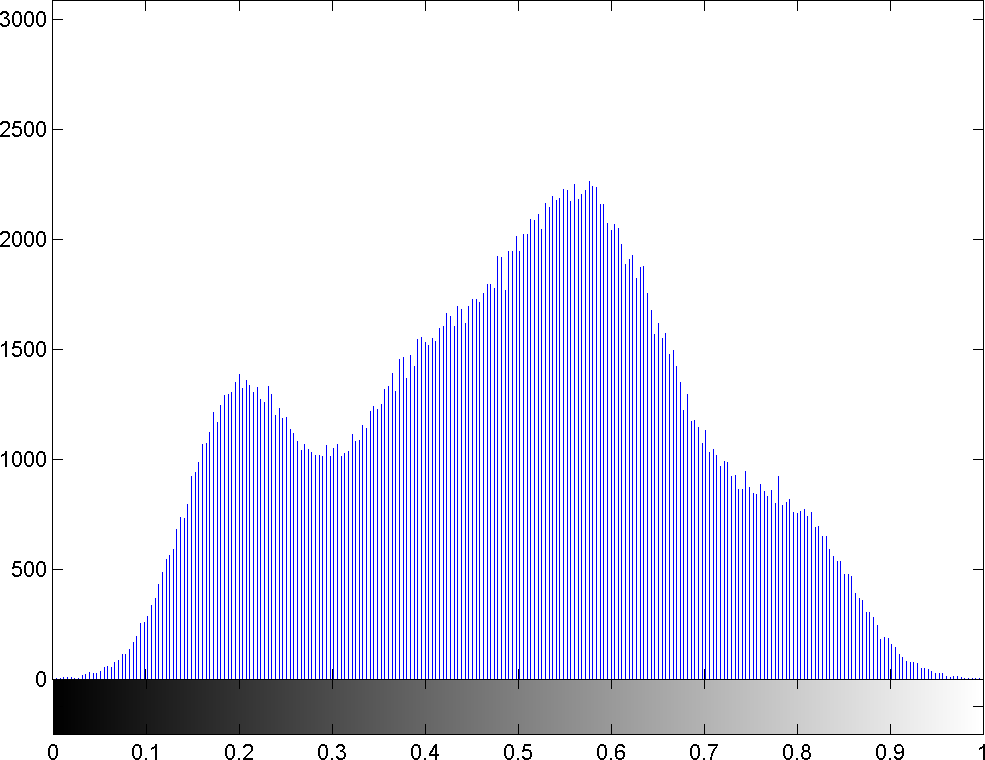
\includegraphics[width=0.45\linewidth]{question3/0_lenaNoisyGauss_hist}
	}
	\caption{Images with Gaussian noise}
	\label{fig:gaussianNoise}
\end{figure}


\clearpage
\subsection{Section1}
\begin{figure}[ht]
\centering
	\subfigure[Denoised image with 3x3 average kernel; PSNR +30.63dB]{
	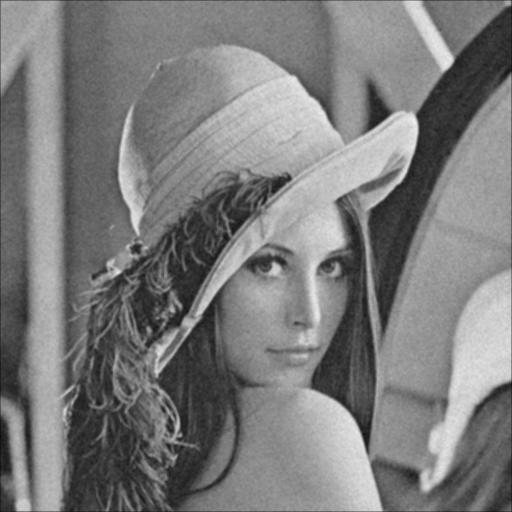
\includegraphics[width=0.45\linewidth]{question3/1_lenaDeNoisyGauss3x3avg}
	}
	\subfigure[Histogram]{
	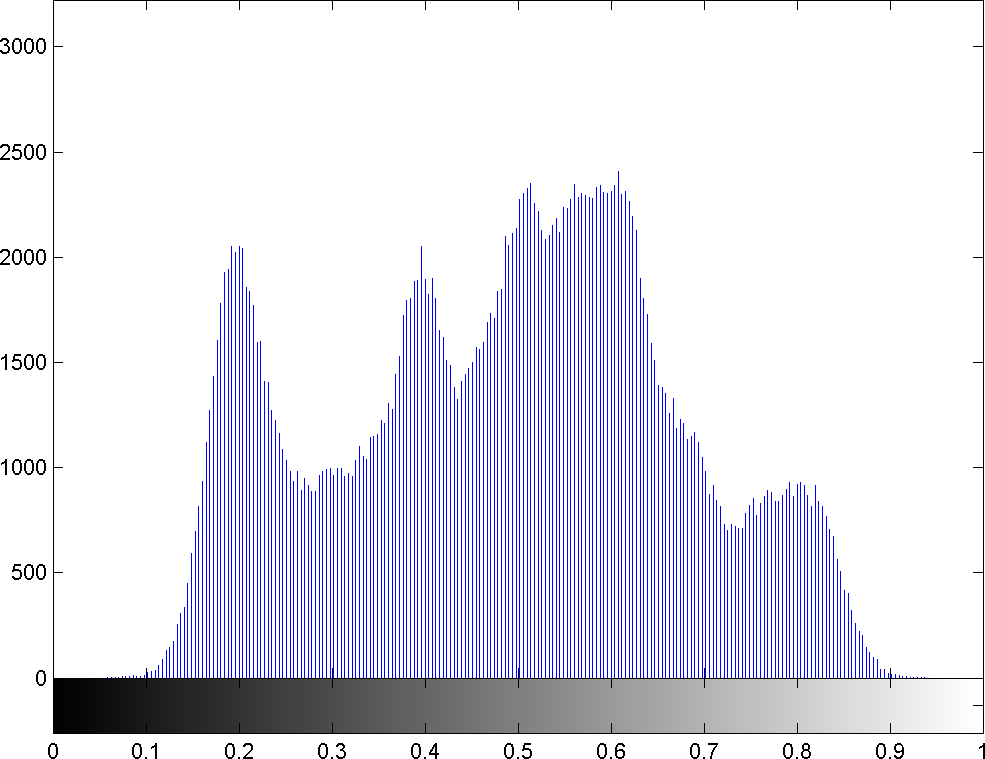
\includegraphics[width=0.45\linewidth]{question3/1_lenaDeNoisyGauss3x3avg_hist}
	}
	
	\caption{Images with Gaussian noise}
	\label{fig:gaussianNoise}
\end{figure}

\clearpage
\subsection{Section2}
\begin{figure}[ht]
\centering
	\subfigure[Denoised image with 7x7 average kernel; PSNR +26.23dB]{
	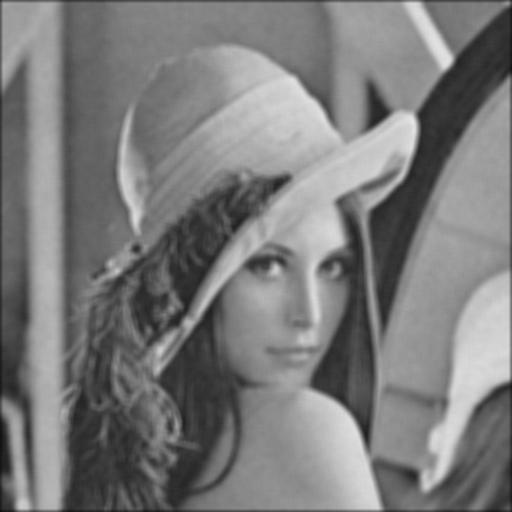
\includegraphics[width=0.45\linewidth]{question3/2_lenaDeNoisyGauss7x7avg}
	}
	\subfigure[Histogram]{
	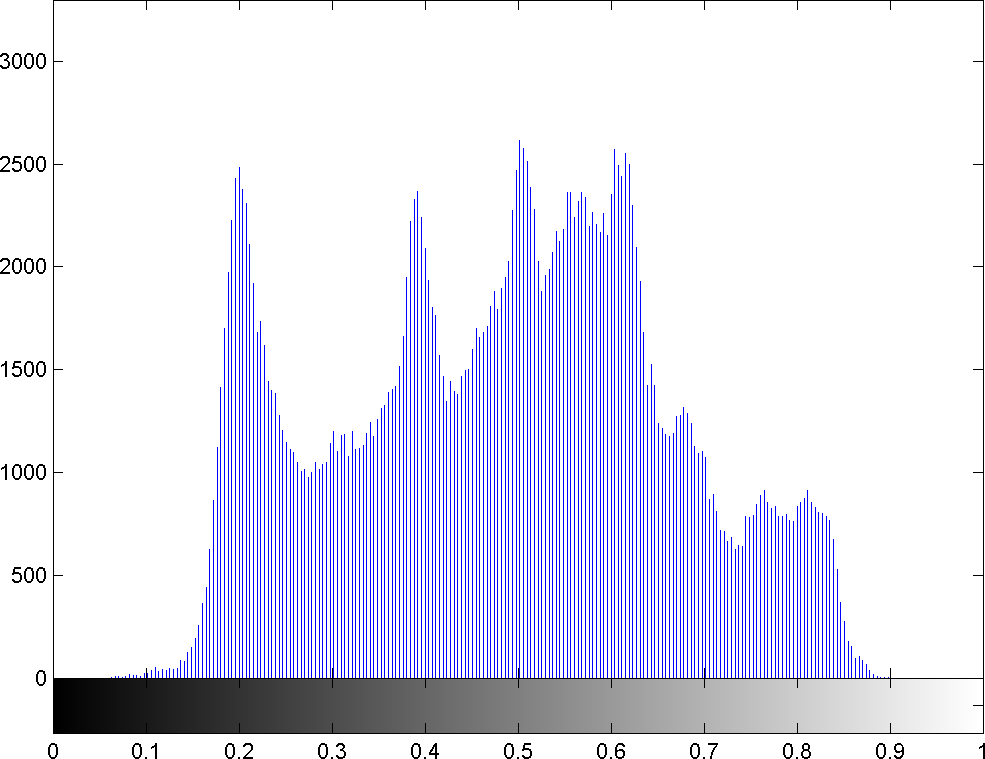
\includegraphics[width=0.45\linewidth]{question3/2_lenaDeNoisyGauss7x7avg_hist}
	}
	
	\caption{Images with Gaussian noise}
	\label{fig:gaussianNoise}
\end{figure}

\clearpage
\subsection{Section3}
\begin{figure}[ht]
\centering
	\subfigure[Denoised image with 7x7 Gaussian kernel; PSNR +30.82dB]{
	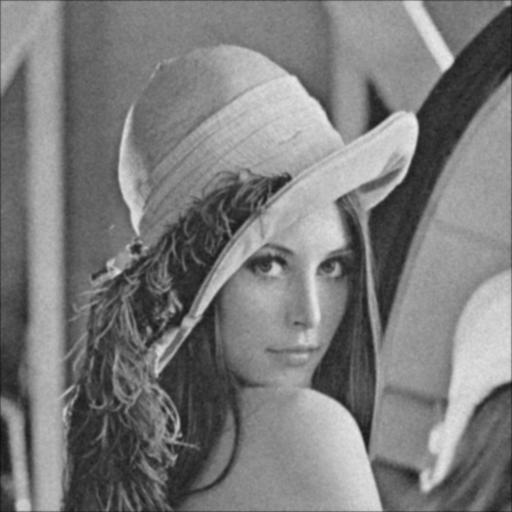
\includegraphics[width=0.45\linewidth]{question3/3_lenaDeNoisyGauss7x7avgGauss}
	}
	\subfigure[Histogram]{
	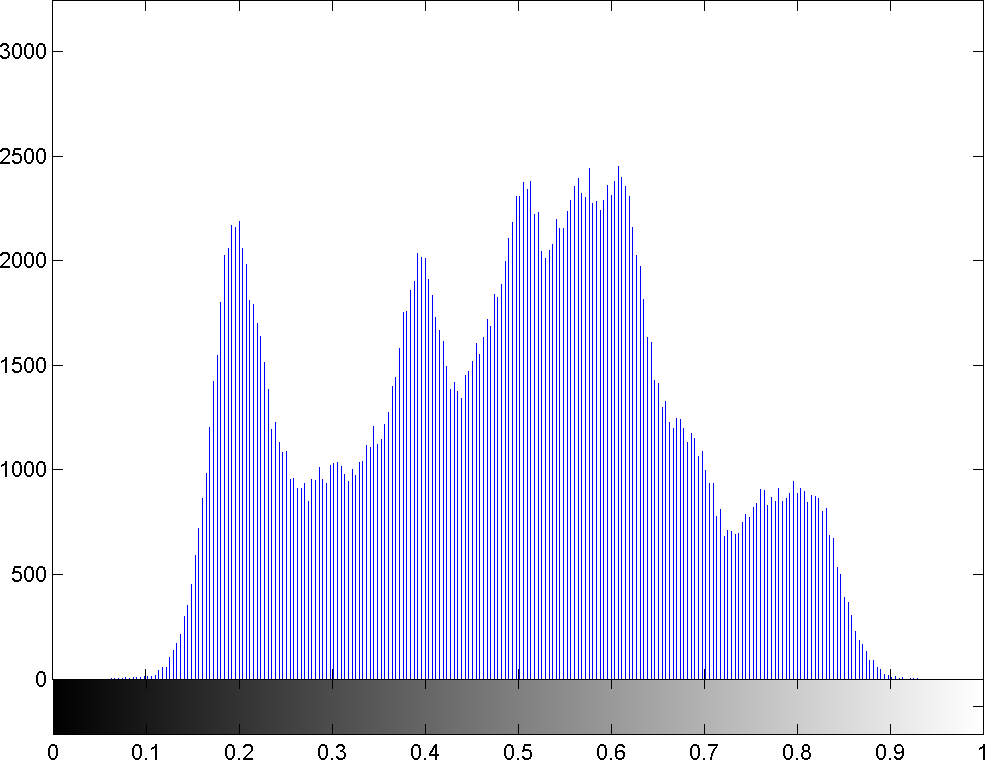
\includegraphics[width=0.45\linewidth]{question3/3_lenaDeNoisyGauss7x7avgGauss_hist}
	}
	
	\caption{Images with Gaussian noise}
	\label{fig:gaussianNoise}
\end{figure}


\clearpage
\subsection{Section4}

\begin{figure}[ht]
\centering
	\subfigure[S\&P noise on original image; PSNR +18.41dB]{
	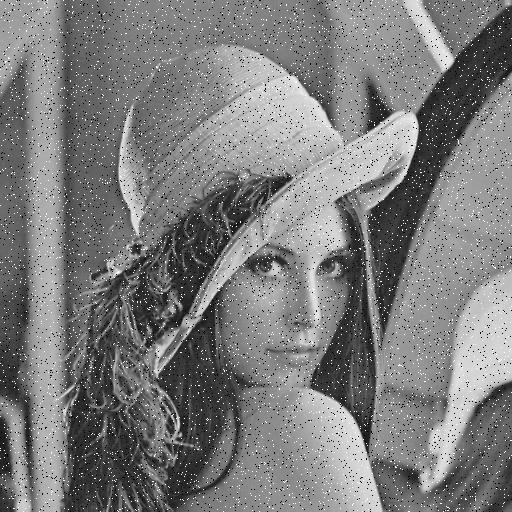
\includegraphics[width=0.45\linewidth]{question3/4_lenaNoisySp}
	}
	\subfigure[Histogram]{
	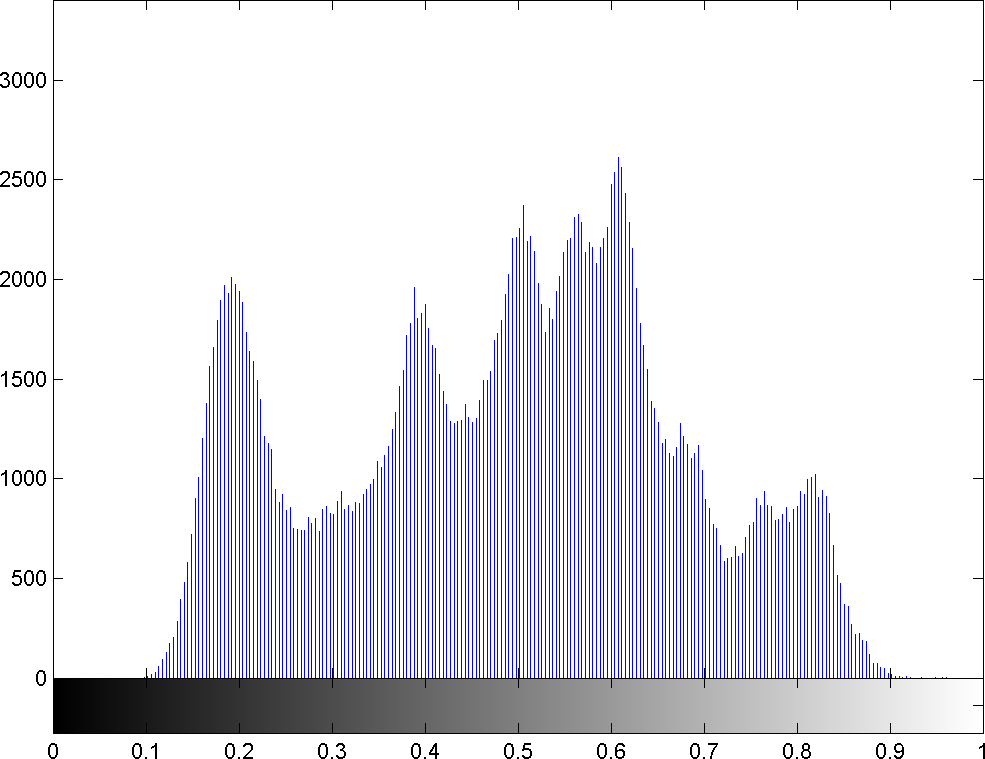
\includegraphics[width=0.45\linewidth]{question3/4_lenaNoisySp_hist}
	}
\end{figure}

\begin{figure}[ht]
\centering	
	\subfigure[S\&P denoised with 7x7 average kernel; PSNR +25.52dB]{
	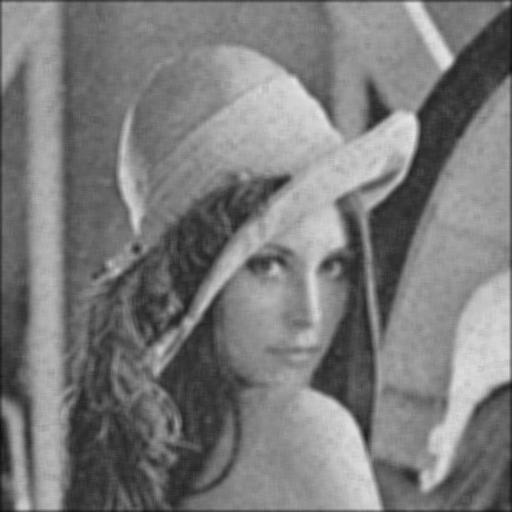
\includegraphics[width=0.45\linewidth]{question3/4_lenaDeNoisySp_7x7Avg}
	}
	\subfigure[Histogram]{
	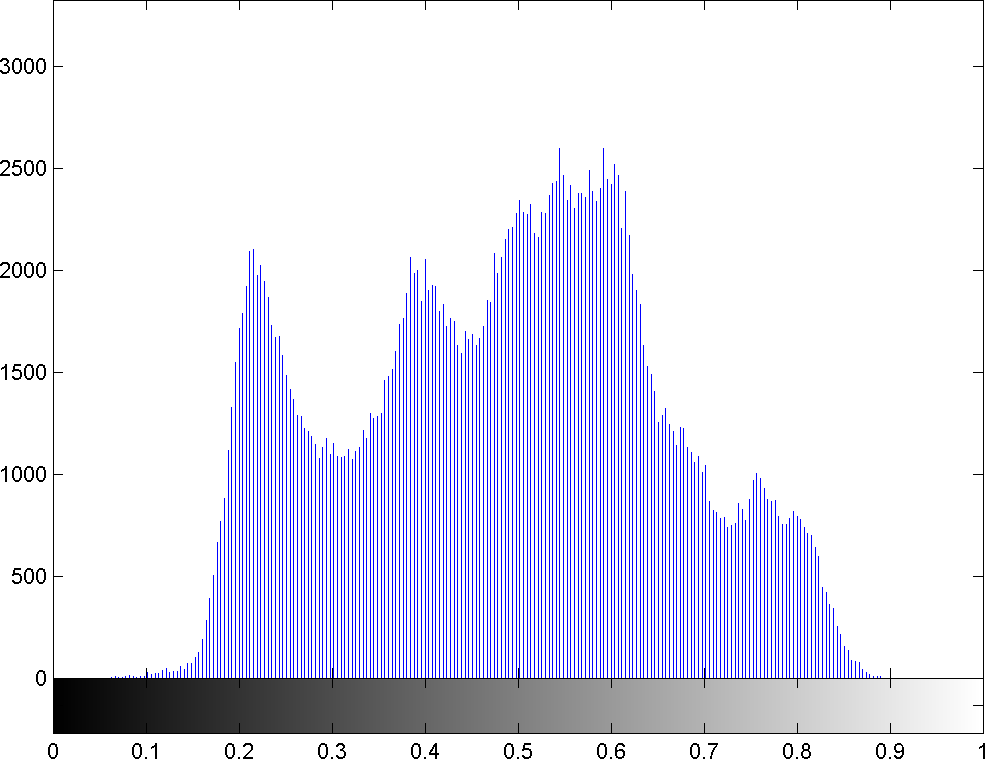
\includegraphics[width=0.45\linewidth]{question3/4_lenaDeNoisySp_7x7Avg_hist}
	}
\end{figure}

\begin{figure}[ht]
\centering
	\subfigure[S\&P denoised with 7x7 Gaussian kernel; PSNR +27.08dB]{
	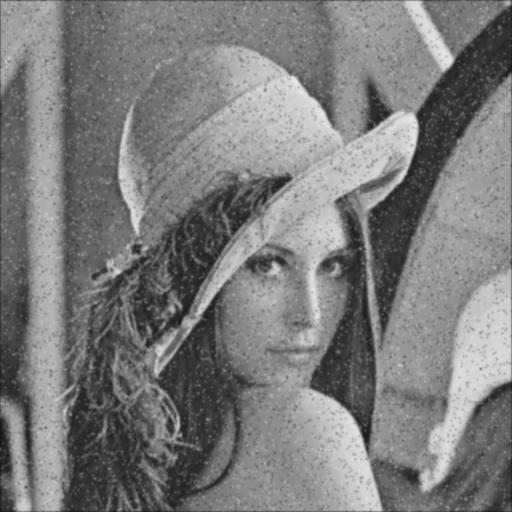
\includegraphics[width=0.45\linewidth]{question3/4_lenaDeNoisySp_7x7AvgGauss}
	}
	\subfigure[Histogram]{
	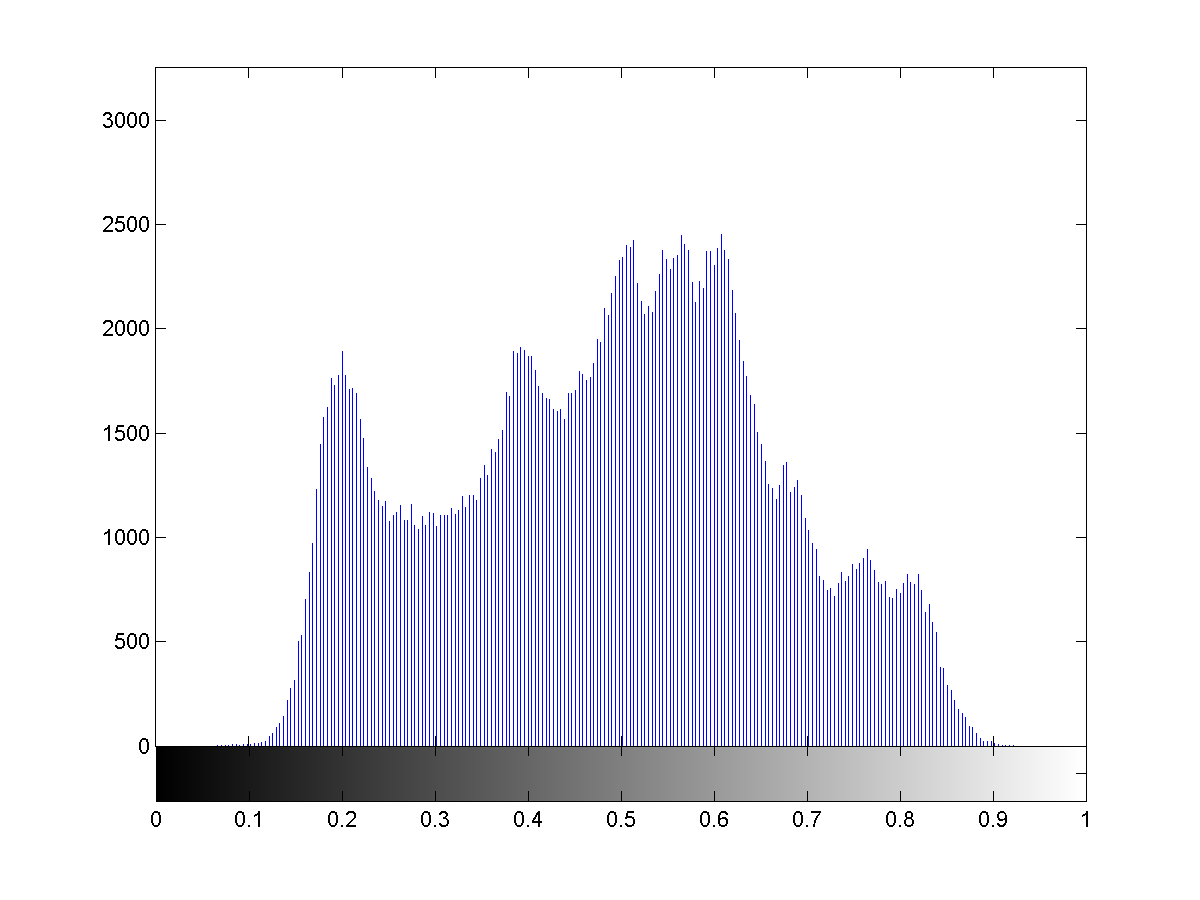
\includegraphics[width=0.45\linewidth]{question3/4_lenaDeNoisySp_7x7AvgGauss_hist}
	}
\end{figure}


\clearpage
\subsection{Section5}

\begin{figure}[ht]
\centering
	\subfigure[S\&P denoised with median filter; PSNR +34.47]{
	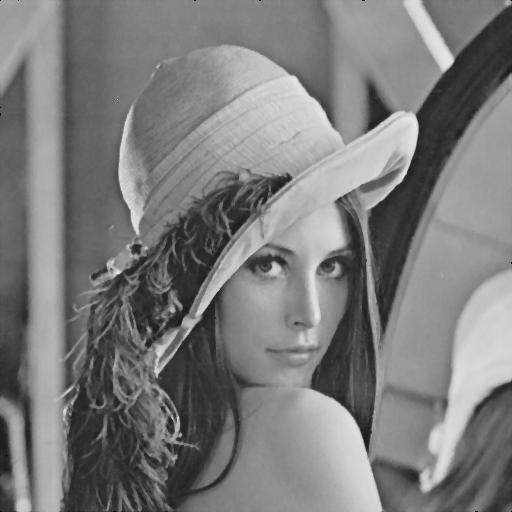
\includegraphics[width=0.45\linewidth]{question3/5_lenaDeNoisyMedian}
	}
	\subfigure[Histogram]{
	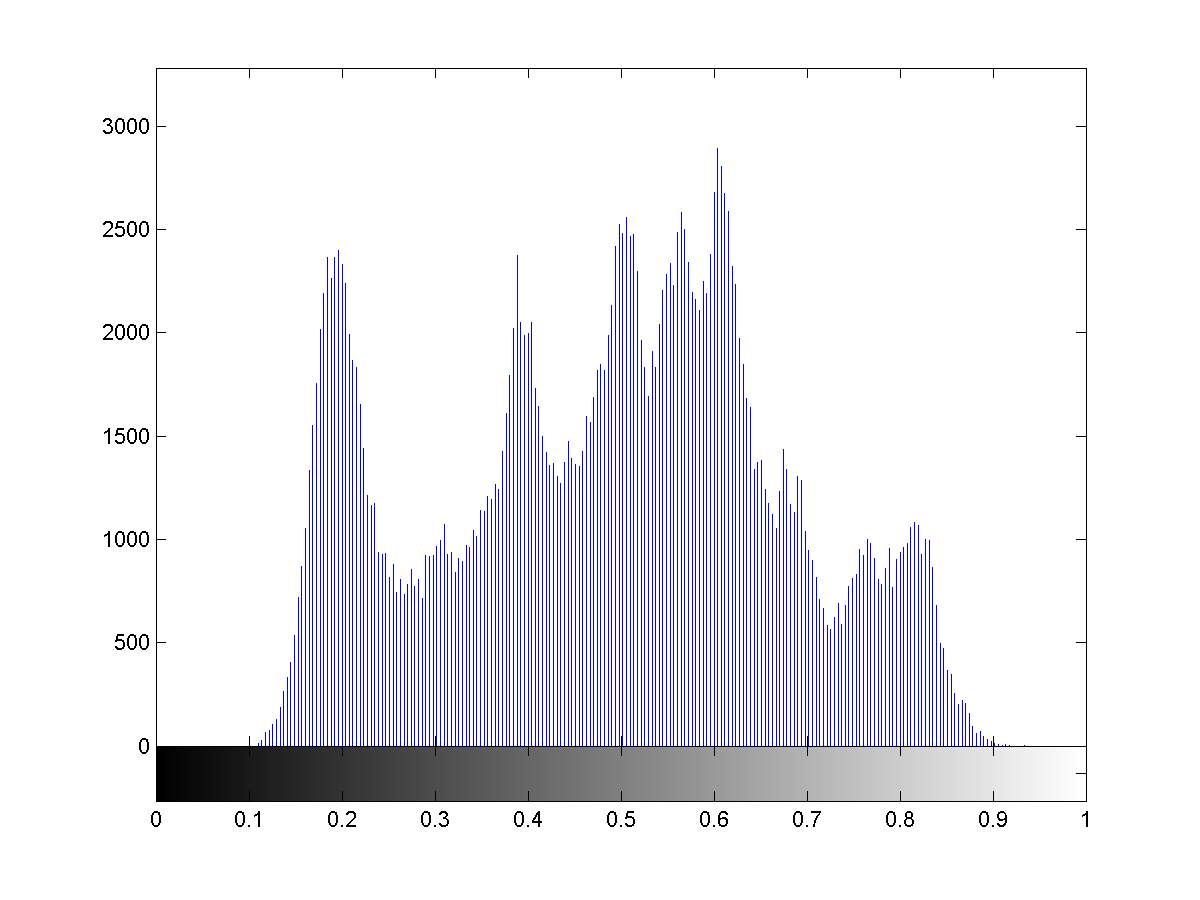
\includegraphics[width=0.45\linewidth]{question3/5_lenaDeNoisyMedian_hist}
	}
\end{figure}

\clearpage


\subsection{Discussion questions}

\subsubsection{Compare the visual difference between the noisy image and the denoised image. How well did it
work? Why? Did the PSNR decrease?}
The denoised image appears blurrier. The denoising worked rather well, as the PSNR is higher in the denoised image. This is because Gaussian is additive noise, and averaging works well at removing additive noise.

\subsubsection{Compare the histograms of the noise-free, noisy, and denoised images. What happened? Why}
The noisy histogram is missing the sharp peaks of the noise free image, instead smoothing it closer to an overall Gaussian distributed shape (due to the additive noise). The averaging filter partially restores this histogram pattern.


\subsubsection{Based on visual quality of the denoised image, what are the benefits and drawbacks associated with
the average filter}
While overall noise is reduced and the PSNR is higher, the image is of reduced visual quality compared to the original (i.e. blurry).


\subsubsection{Compare the visual difference between the denoised image from the 7x7 filtering kernel and the
denoised image from the 3x3 filtering kernel. Are there any differences? Why? Did the PSNR
decrease? Why}
The 7x7 filtered image is even blurrier than the 3x3 filtered one. This is because it averages over a wider area. The PSNR also decreased, with the PSNR now slightly less than that of the noisy image. This is because by taking a wider averaging window, high frequency elements such as edges are further suppressed.


\subsubsection{Compare the histograms of the two denoised images. What are the differences? Why}
The histogram of the 7x7 has sharper peaks than the 3x3, more closely mirroring that of the original noiseless image. This is because


\subsubsection{Based on visual quality of the denoised image, what are the benefits and drawbacks associated with
using a larger window size?}
While the noise is basically gone from the image, it is extremely blurry; many fine details (especially edges) are lost.


\subsubsection{Compare the visual difference between the denoised image from the Gaussian filtering kernel and the
denoised images from the averaging filter kernels. Are there any differences? Why? Did the PSNR
decrease? Why}
The Gaussian filtered image is less blurry than the two averaging filtered images. Finer details are better preserved. This is because with the Gaussian kernel, pixels further away from the centre are weighted less, unlike the uniform averaging of the averaging kernel.


\subsubsection{Compare the histograms of the denoised image using the Gaussian filtering kernel and the denoised
images from the averaging filter kernels. What are the differences? Why?}
The sharp peaks of seen in the 7x7 averaging filter are less pronounced in the Gaussian filter. 


\subsubsection{Based on visual quality of the denoised image, what are the benefits and drawbacks associated with
using a Gaussian kernel as opposed to an averaging kernel?}
The Gaussian kernal results in a less blurry image than the averaging kernal.


\subsubsection{How does the averaging filter and Gaussian filtering methods perform on the noisy image in terms of
noise reduction? Explain in terms of visual quality as well as PSNR. Why do we get such results?}
They all result in blurrier images which have a higher PSNR. This happens because



\subsubsection{Compare the histograms of the denoised images with that of the noisy image. What characteristics
are present in all of the histograms? Why?}
All the histograms of denoised images have more, sharpened peaks. This is because



\subsubsection{How does the denoised image produced using the median filter compare with the denoised images
produced using averaging filter and Gaussian filtering methods? Explain in terms of visual quality
as well as PSNR. Why do we get such results with median filter when compared to the other spatial
filtering methods?}
The median filter produces a superior quality image compared to the gaussian and averaging filters. The PSNR is also significantly higher. We get such results with the median filter because by taking the median value, excessive high/low intensities due to noise do not get taken into account. With the averaging/gaussian filters, these get averaged into the denoised image.
